\documentclass[11pt,a4paper]{article}
\usepackage[utf8]{inputenc}
\usepackage[T1]{fontenc}
\usepackage[spanish]{babel}
\usepackage[margin=2.5cm]{geometry}
\usepackage{longtable}
\usepackage{array}
\usepackage{graphicx}
\setlength{\parindent}{0pt}
\setlength{\parskip}{0.6em}

\begin{document}

\textbf{Declaración:} Esta es la transcripción fiel de la prueba escrita a mano el 18/11/2026 las fotografías de las hojas están en el anexo.

\bigskip
\hrule
\bigskip

Nombres: Luis Yepez

Fecha: 18/11/2026

Examen práctico Ingeniería de Requisitos

Caso de estudio: Sistema de Monitoreo de la Cadena de Frío <<FRÍO VAC>>

T1. Conceptos aplicados al caso \hfill D1*10\%

a) Explique con sus palabras qué es un requisitos según ISO/IEC/IEE 29148 y, con esa explicación, decida si E7 Y E12 son requisitos del producto FRÍOVAC. Justifique cada decisión en una o dos líneas.

Un requisito es una función que  un sistema o software debe realizar.

E7 y E12 no son requisitos de FRIOVAC, E7 menciona que solo anotan la temperatura manualmente en una hoja, no se pide automatizar o algo parecido, mientras que E12 es la obtención de información, son 16 entrevistas que se harán por videollamada.

b) Expliqué qué describe la especificación de los interesados(SIRS) la especificación de requisitos del sistema (SyRS) y la especificación de requisitos del software (SRS) en este proyecto. Para cada una dé un enunciado del insumo A que iría en ella y diga por qué.

Especificación de los interesados: El sistema generará en formato PDF el informe mensual de temperaturas (durante cortes) de cada establecimiento.
¿Por qué?: La coordinadora de inmunizaciones está interesada por saber las temperaturas de sus establecimientos cada mes.

\clearpage

Especificación de requisitos del sistema: El sistema deberá seguir registrando las lecturas del temperatura durante cortes de energía eléctrica de hasta 8 horas.
¿Por qué?: Aclara que de alguna forma el sistema obligatoriamente debe funcionar incluso si hay cortes de energía.

Especificación de requisitos del software: <<Necesitamos enterarnos de inmediato cuando una refrigeradora se salga del rango, aunque sea de madrugada.>>
¿Por qué?: Solicitan que el software pueda enviar notificaciones o avisos cada vez que una refrigeradora salga de su rango sin importar la hora que sea.

c) Para cada hecho H1 a H5 indique a qué actividad del proceso de IR, corresponde (elicitación, análisis y negociación, especificación, validación o gestión) y sí en el marco de Pohl es una actividad centra o transversal.

H1: Pertenece a la elicitación y es una actividad central.

H2: Pertenece a análisis y negociación, y es una actividad transversal.

H3: Pertenece a especificación, ya que coloca identificadores, además es una actividad central.

H4: Pertenece a análisis y negociación, ya que deben aclarar qué hacen durante los cortes de energía, es una actividad central.

H5: Pertenece a validación y gestión, y es una actividad central.

\clearpage

T2- Clasificación y auditoría \hfill D2*30\%

a) Clasificación. Dibuje una tabla con las columnas ID, tipo, Documento y justificación, y complétela para E1 a E12. Tipo: funcional; no funcional(diga la característica de ISO/IEC 25010:2023); restricción; requisito de dominio; requisito de proceso; o no es requisito. Documento: StRS, SyRS, SRS o ninguno de ellos (diga dónde se registra entonces). La justificación cabe en una línea.

\medskip
\begin{longtable}{|p{1.2cm}|p{3.0cm}|p{3.0cm}|p{6.2cm}|}
\hline
ID & Tipo & Documento y & Justificación \\ \hline
E1 & Funcional & SRS & El software debe notificar. \\ \hline
E2 & Dominio & SyRS/SRS & Regla de farmacEuticos. \\ \hline
E3 & Restricción & SyRS & Uso obligatorio del sensor. \\ \hline
E4 & Restricción & StRS & LImite temporal de pagos. \\ \hline
E5 & Funcional & SRS & Debe generar informes mensuales. \\ \hline
E6 & No funcional & SyRS & Capacidad de funcionamiento. \\ \hline
E7 & No es requisito & Nada & Solo describe un procedimiento. \\ \hline
E8 & No funcional & SRS & Tiempo de respuesto del sistema. \\ \hline
E9 & Restricción & SyRS & Obligación técnico para el uso. \\ \hline
E10 & Funcional & SRS & Control de permisos de usuarios. \\ \hline
E11 & No funcional & SRS & Tiempo de aprendizaje de usuario. \\ \hline
E12 & Proceso & Ninguno & Organización para buscar información. \\ \hline
\end{longtable}

\clearpage

(b) Auditoría. Dibuje una tabla con las columnas ID, término o construcción problemática. Caracteristíca de 29148 que incumple, propiedad SMART que incumple y Justificación, y complétela para B1 a b6. Si un requisito está bien formado, digalo y explique porqué con la clausula 5.2.4

\medskip
\begin{longtable}{|p{1.5cm}|p{3.4cm}|p{4.2cm}|p{4.2cm}|}
\hline
ID & Término & Característica & Propiedad SMART \\ \hline
B1 & & & \\ \hline
\end{longtable}

\clearpage

\appendix
\section*{Anexo: fotografías de las hojas}

\begin{center}
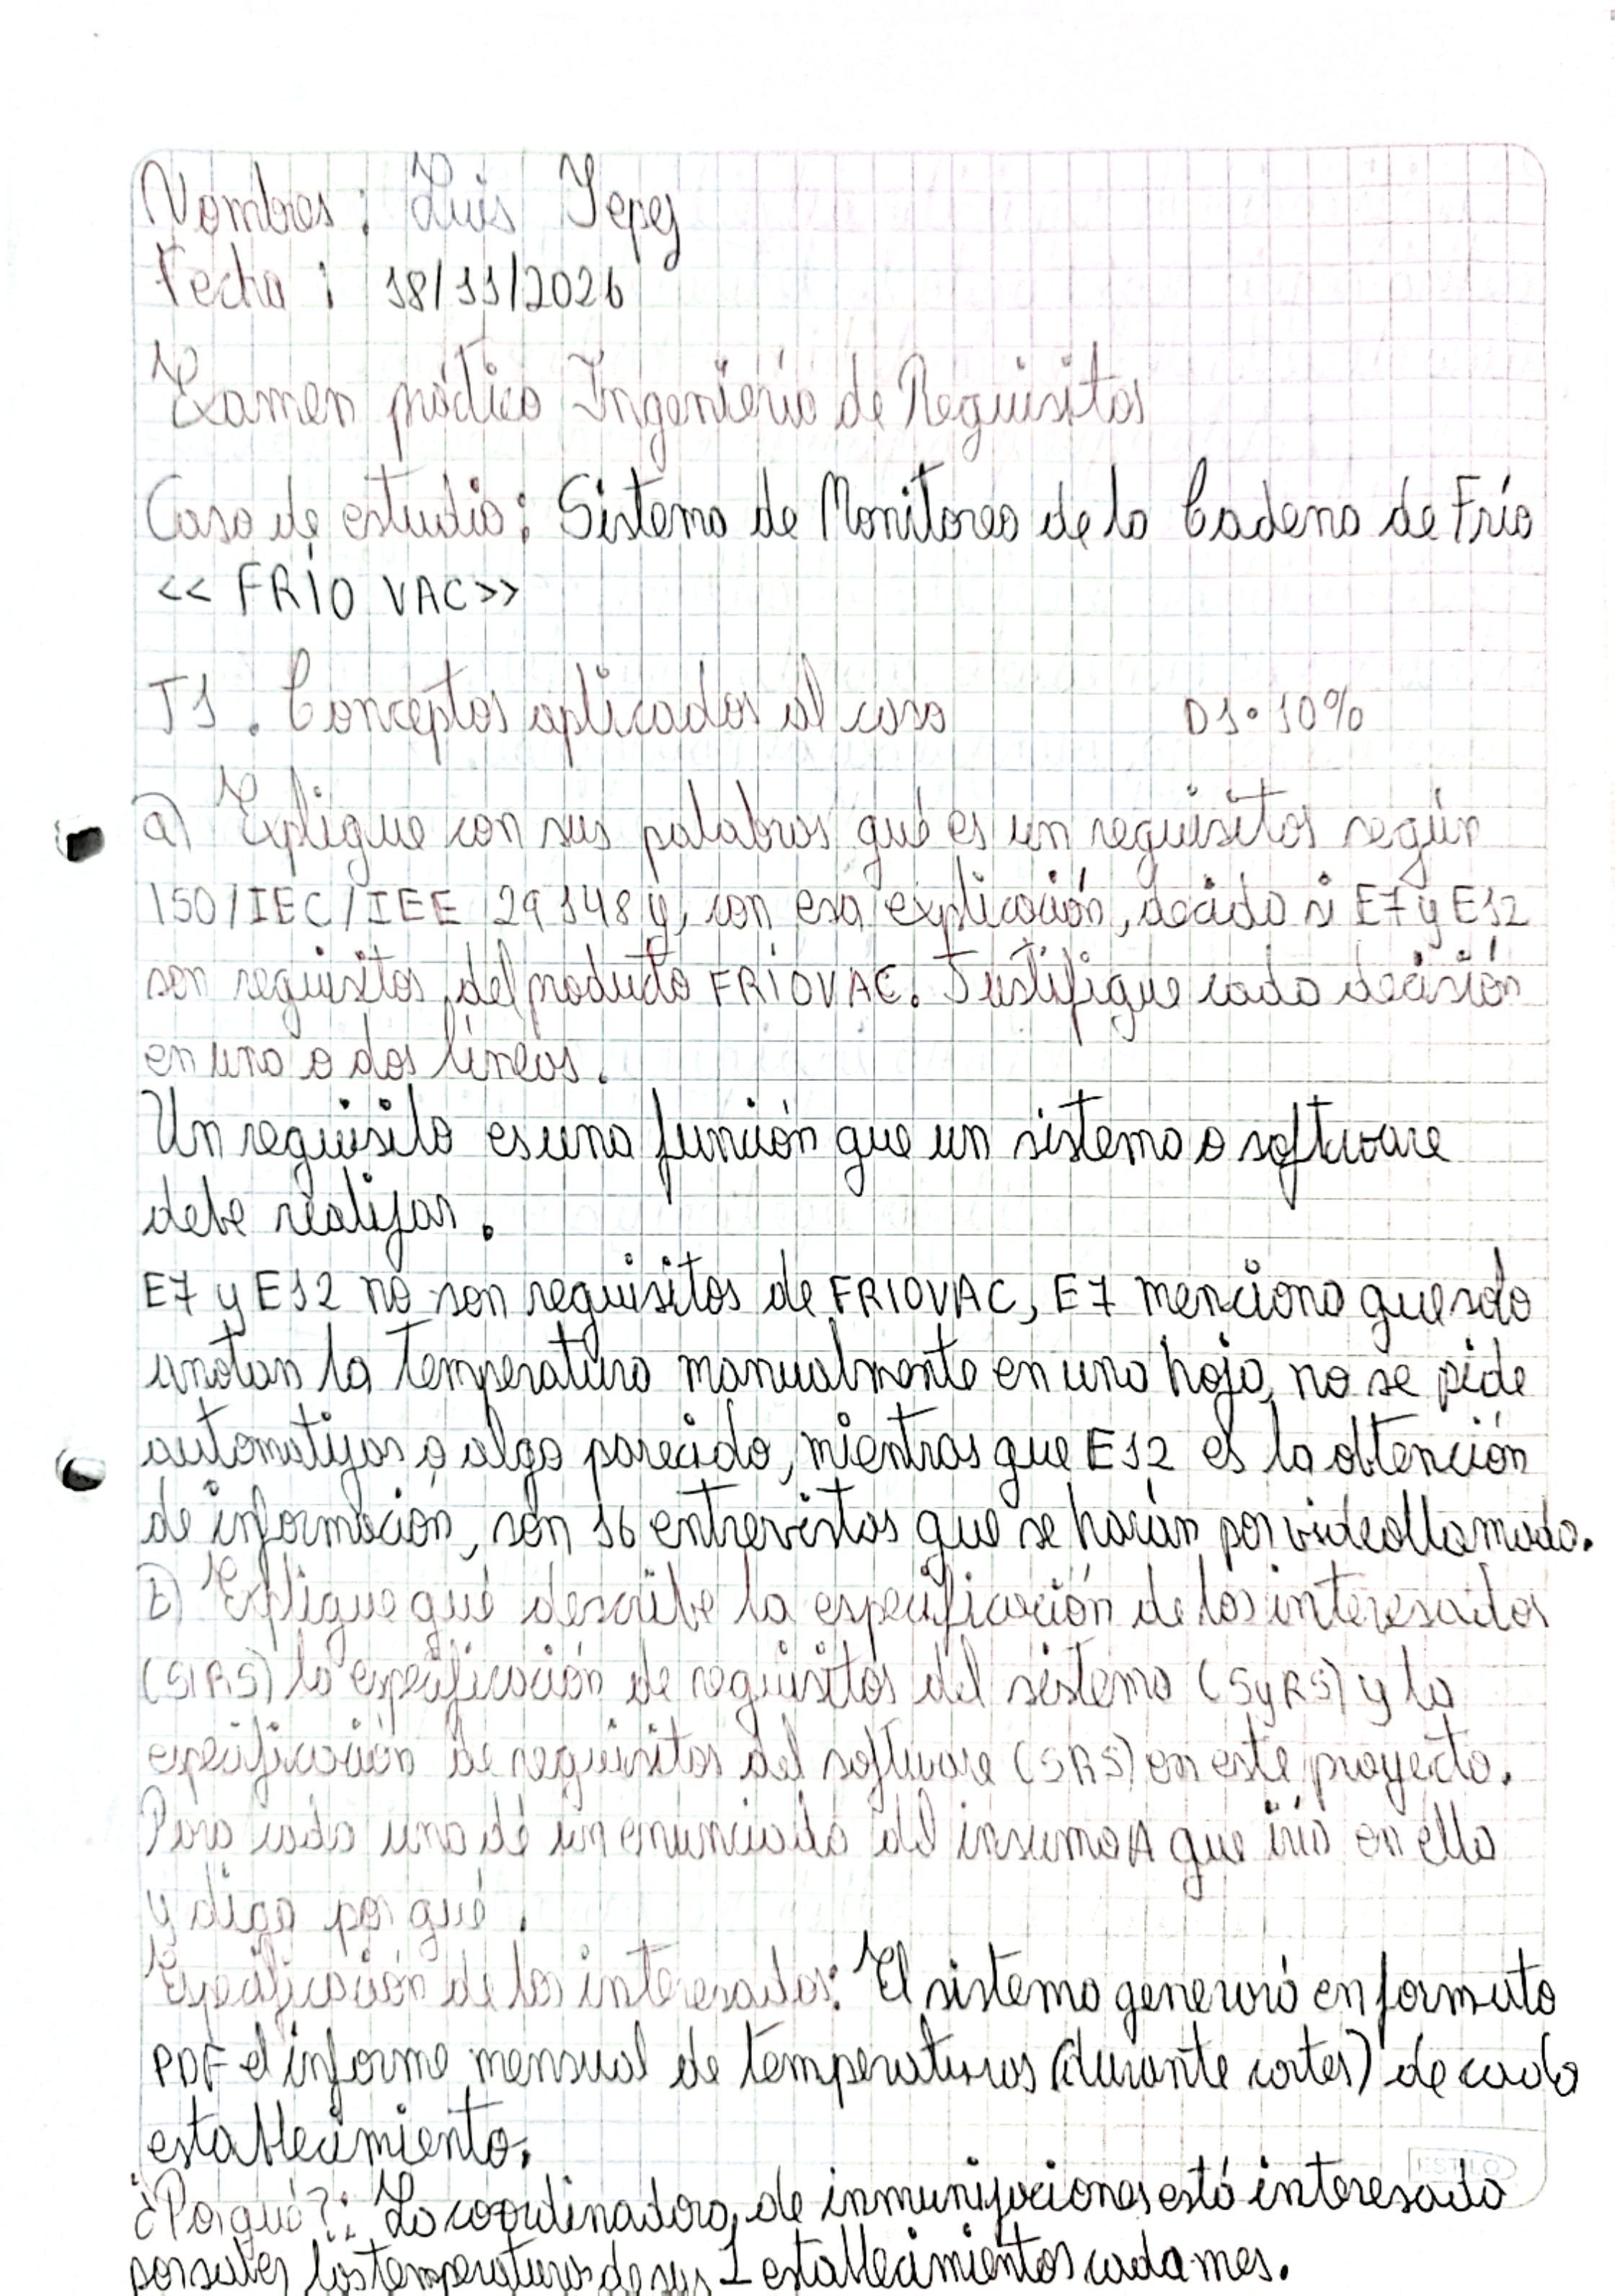
\includegraphics[width=0.85\textwidth,height=0.42\textheight,keepaspectratio]{evidencias/hoja-01.jpg}\\[1em]
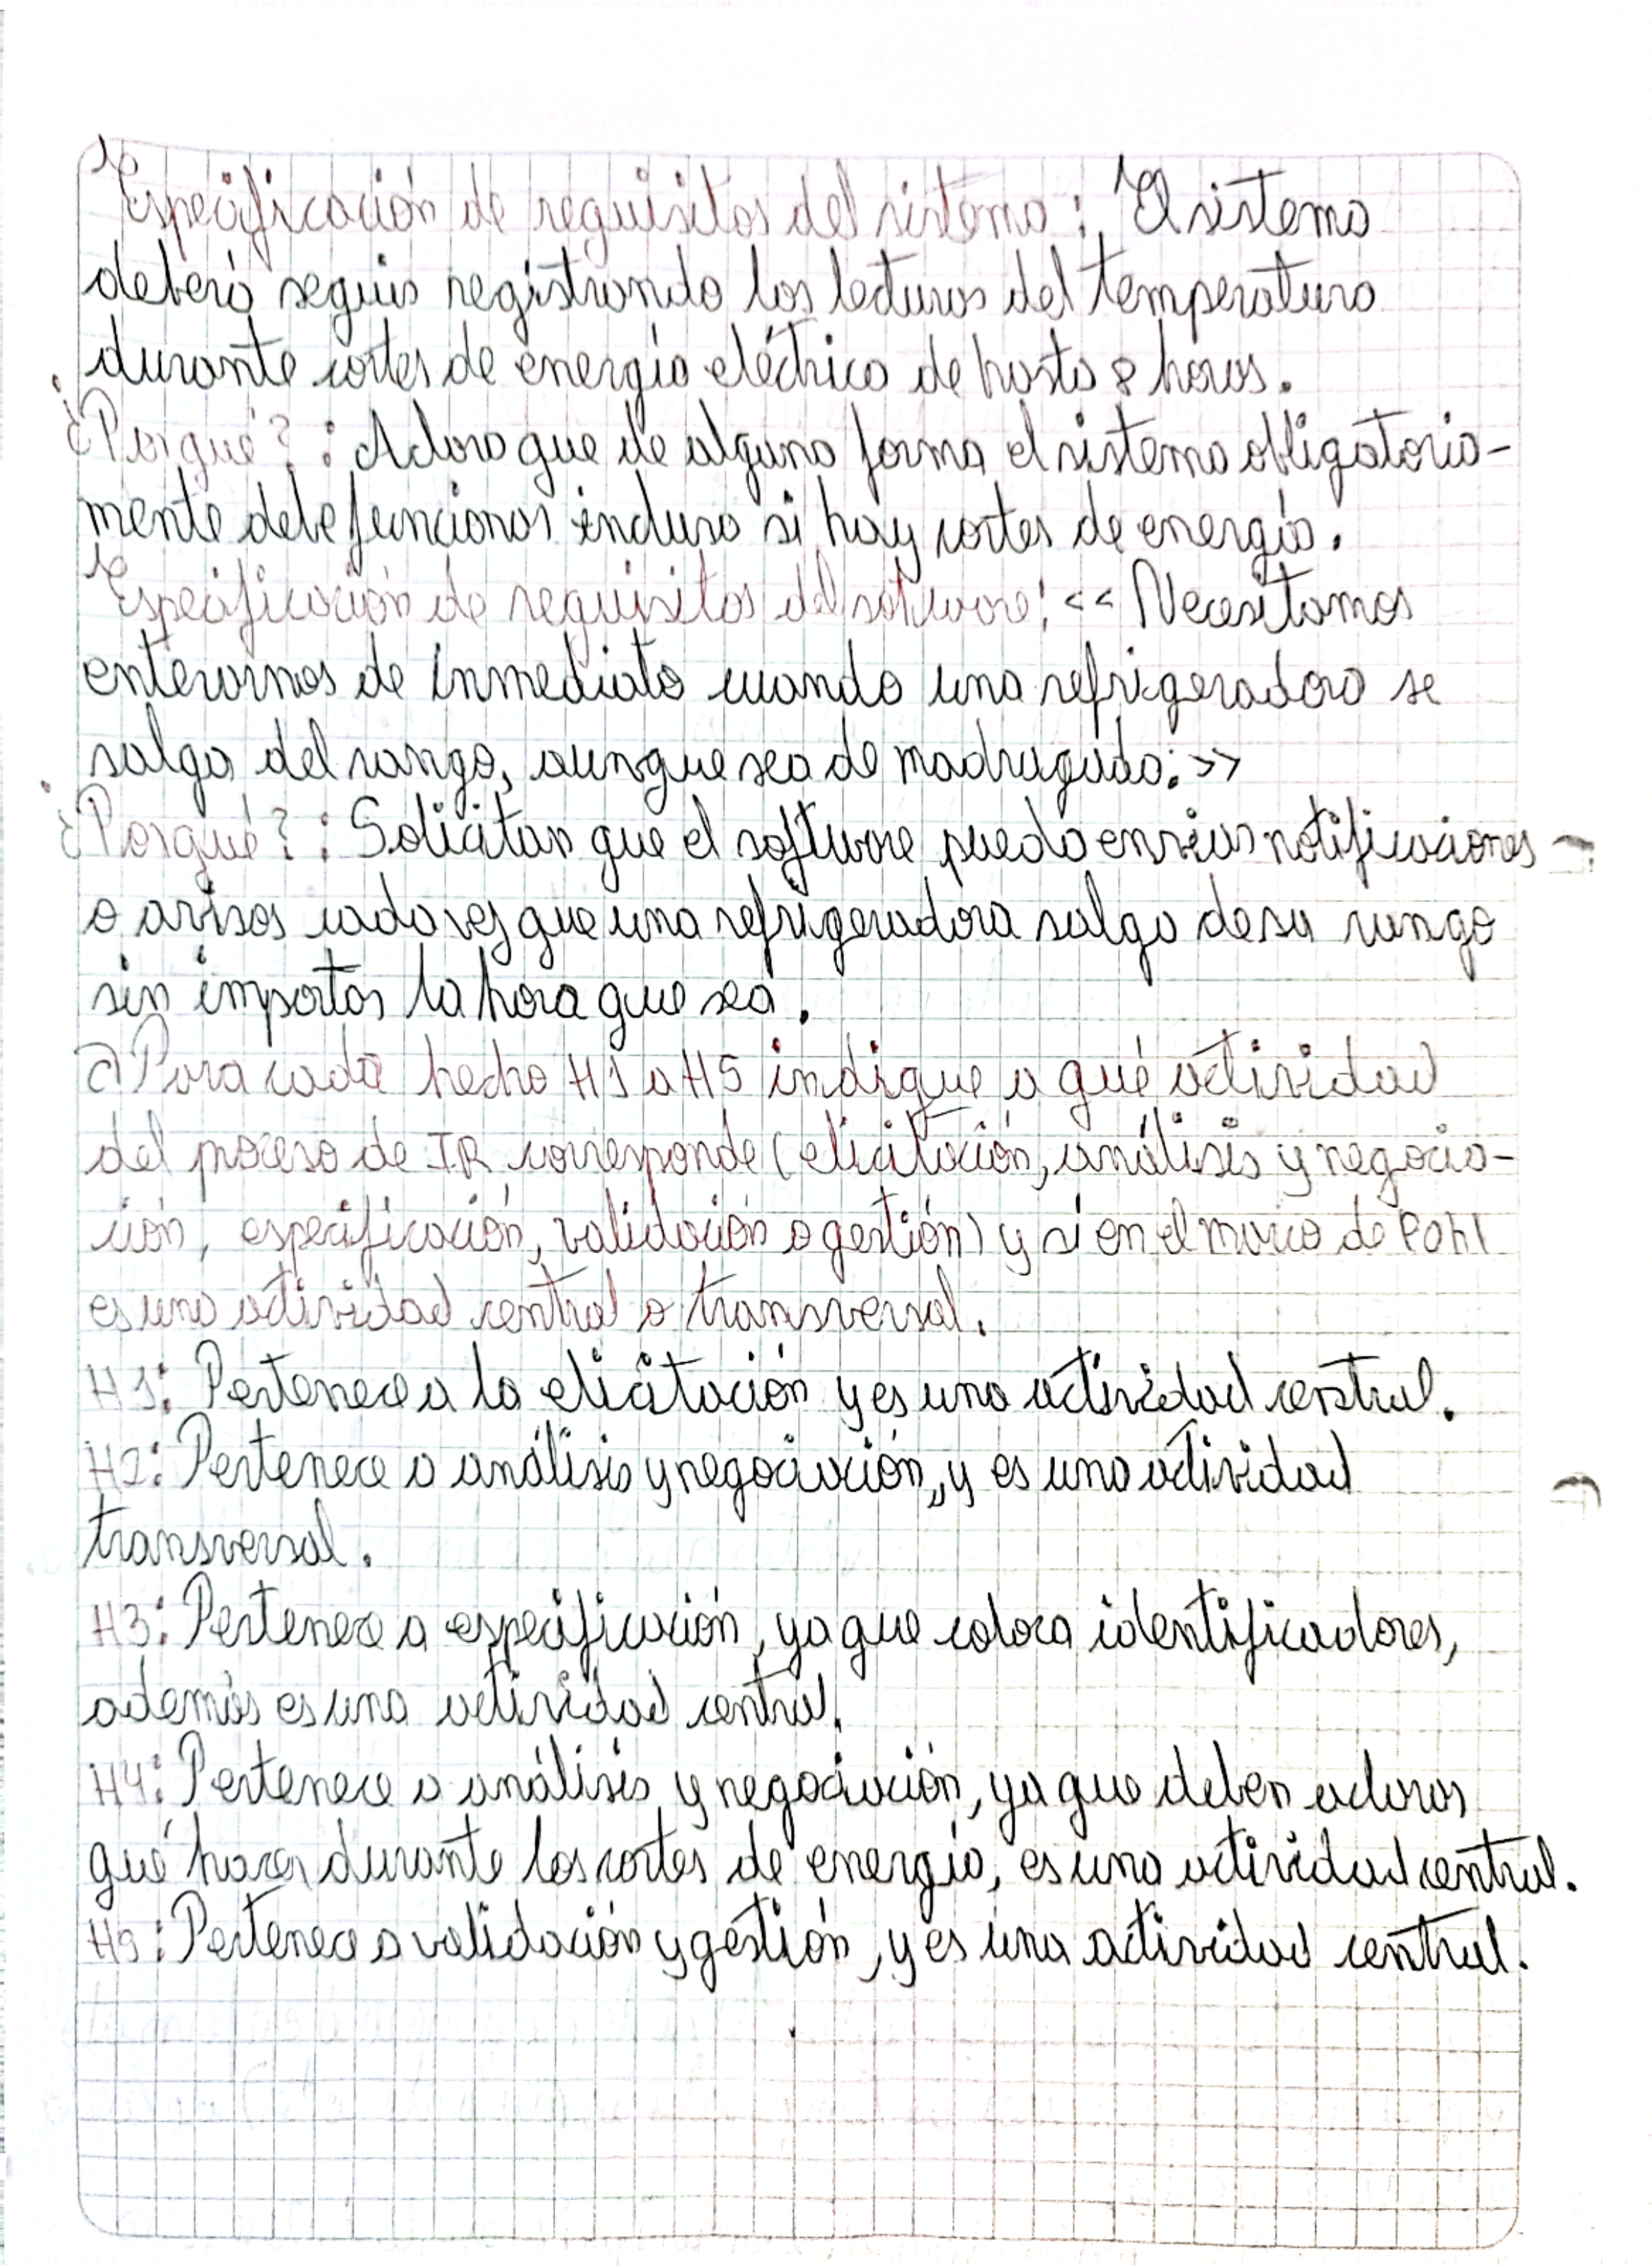
\includegraphics[width=0.85\textwidth,height=0.42\textheight,keepaspectratio]{evidencias/hoja-02.jpg}
\end{center}
\clearpage
\begin{center}
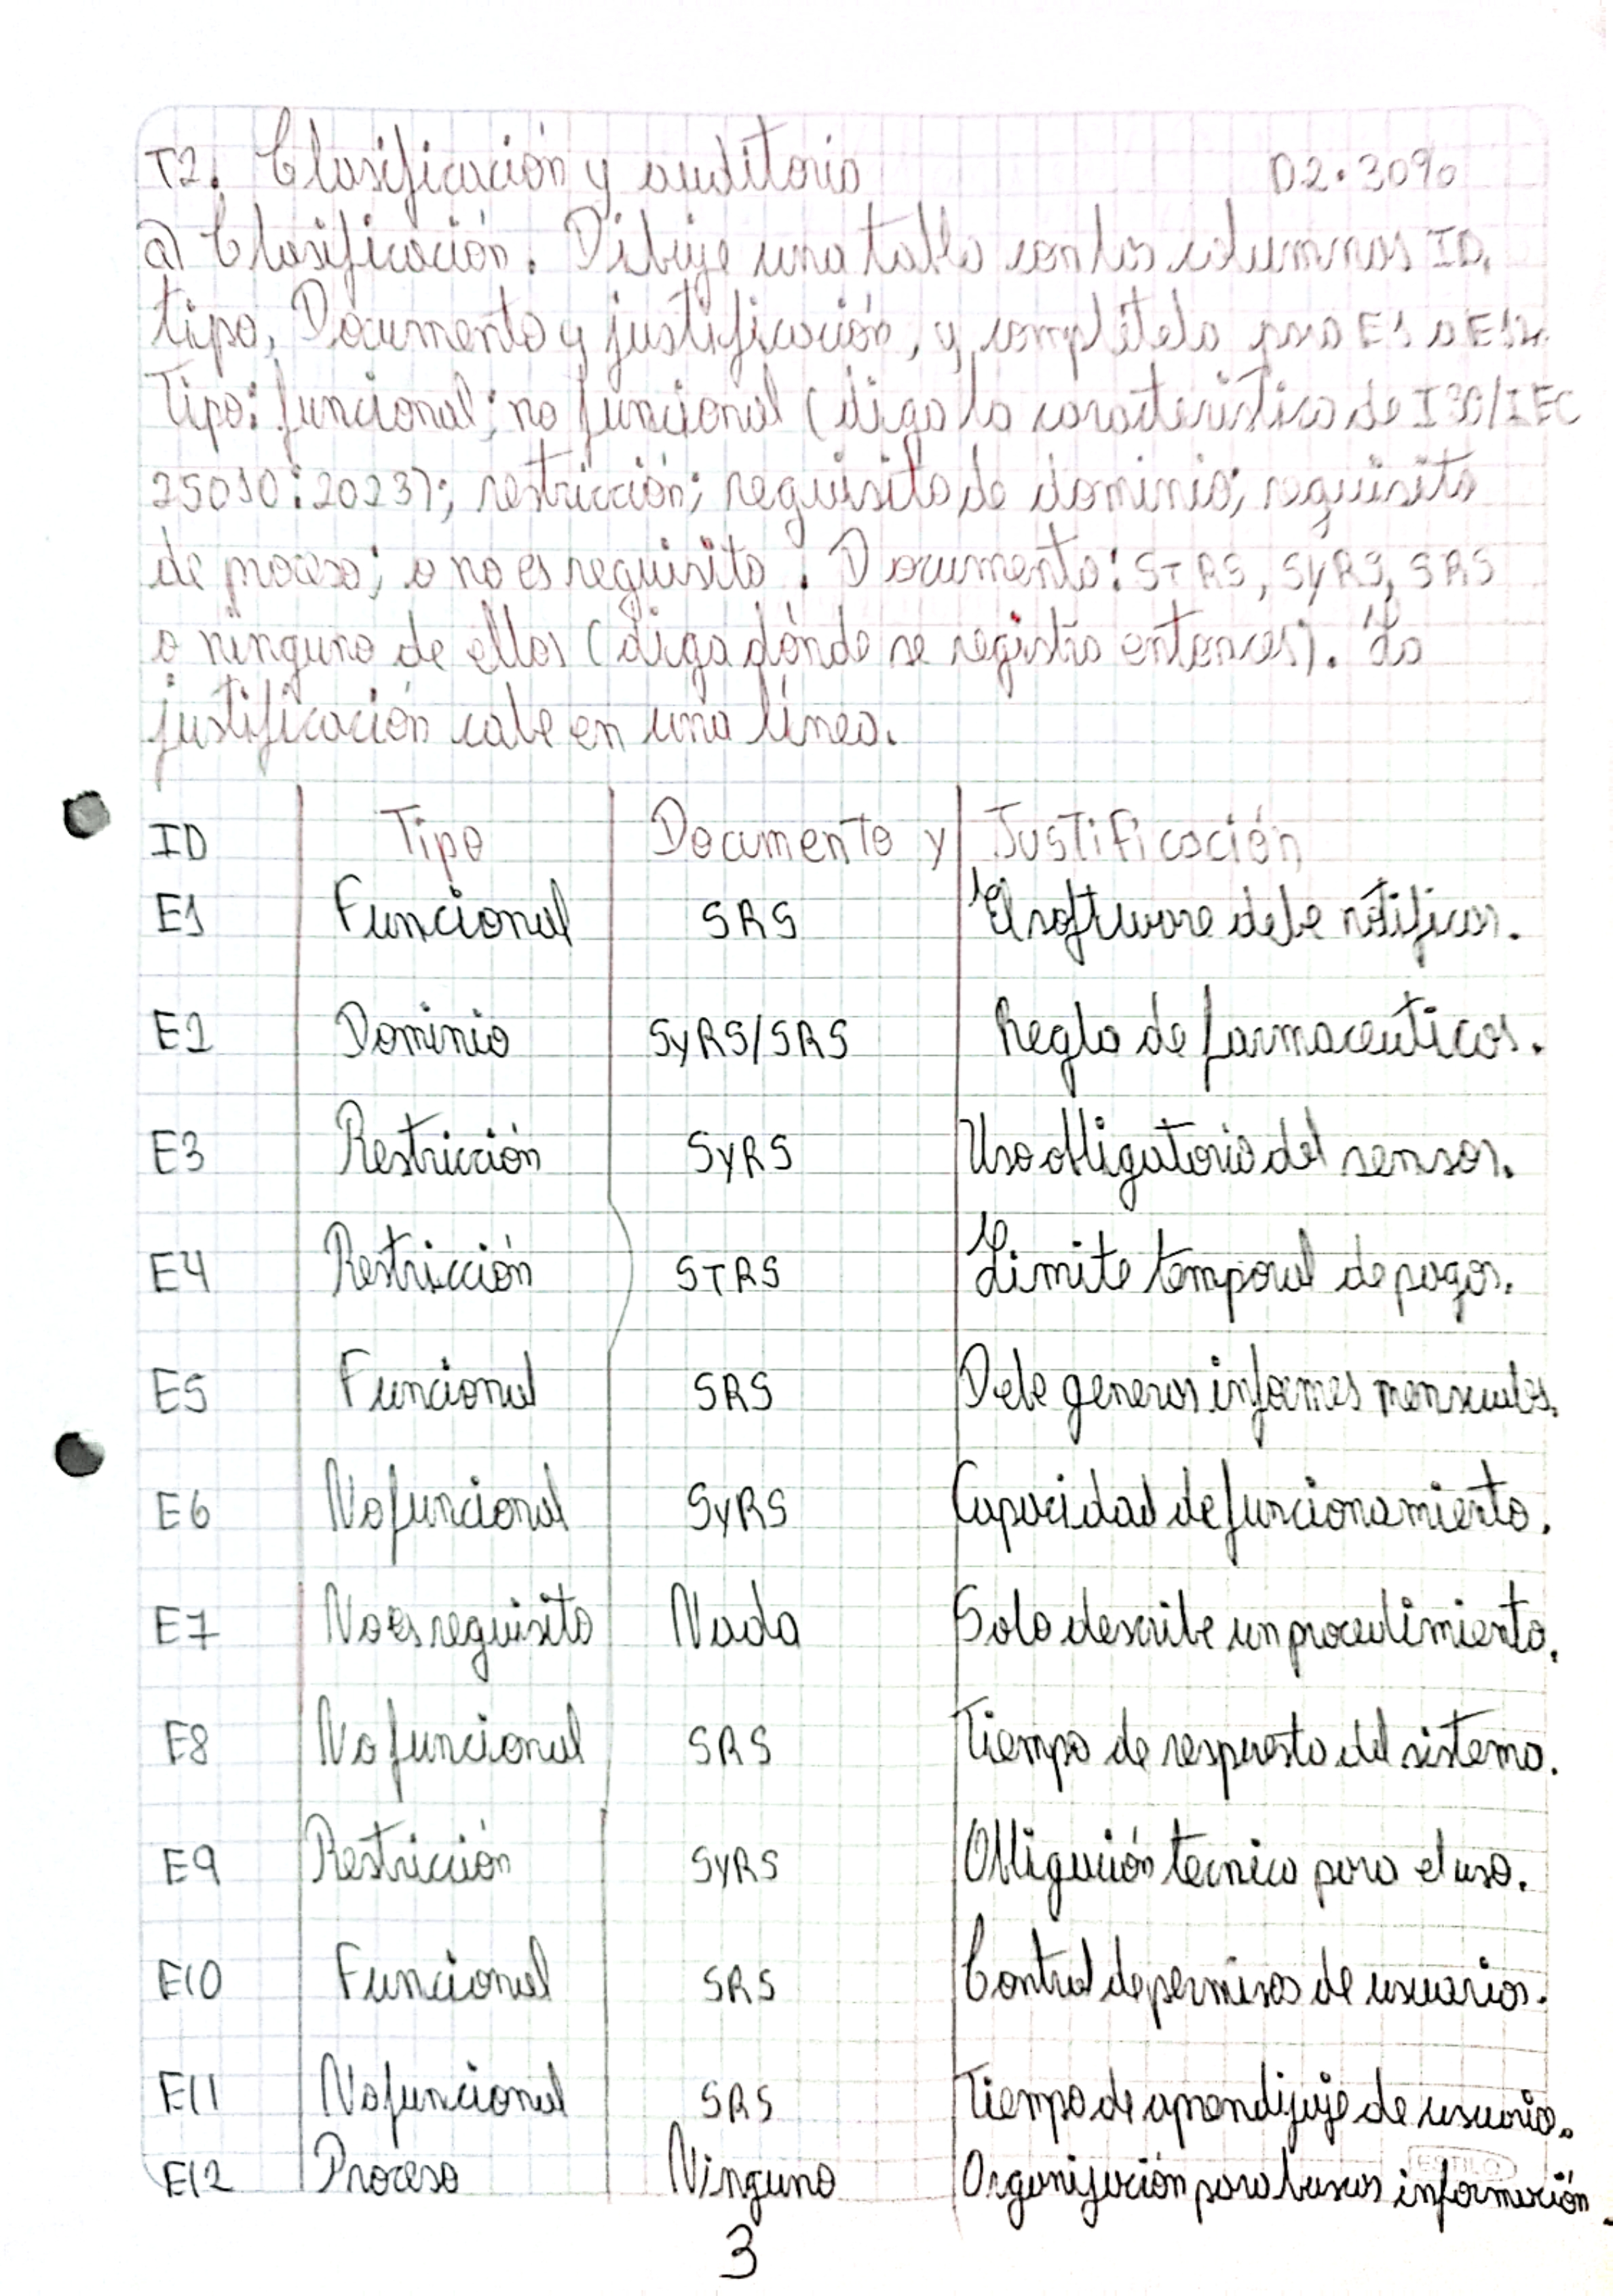
\includegraphics[width=0.85\textwidth,height=0.42\textheight,keepaspectratio]{evidencias/hoja-03.jpg}\\[1em]
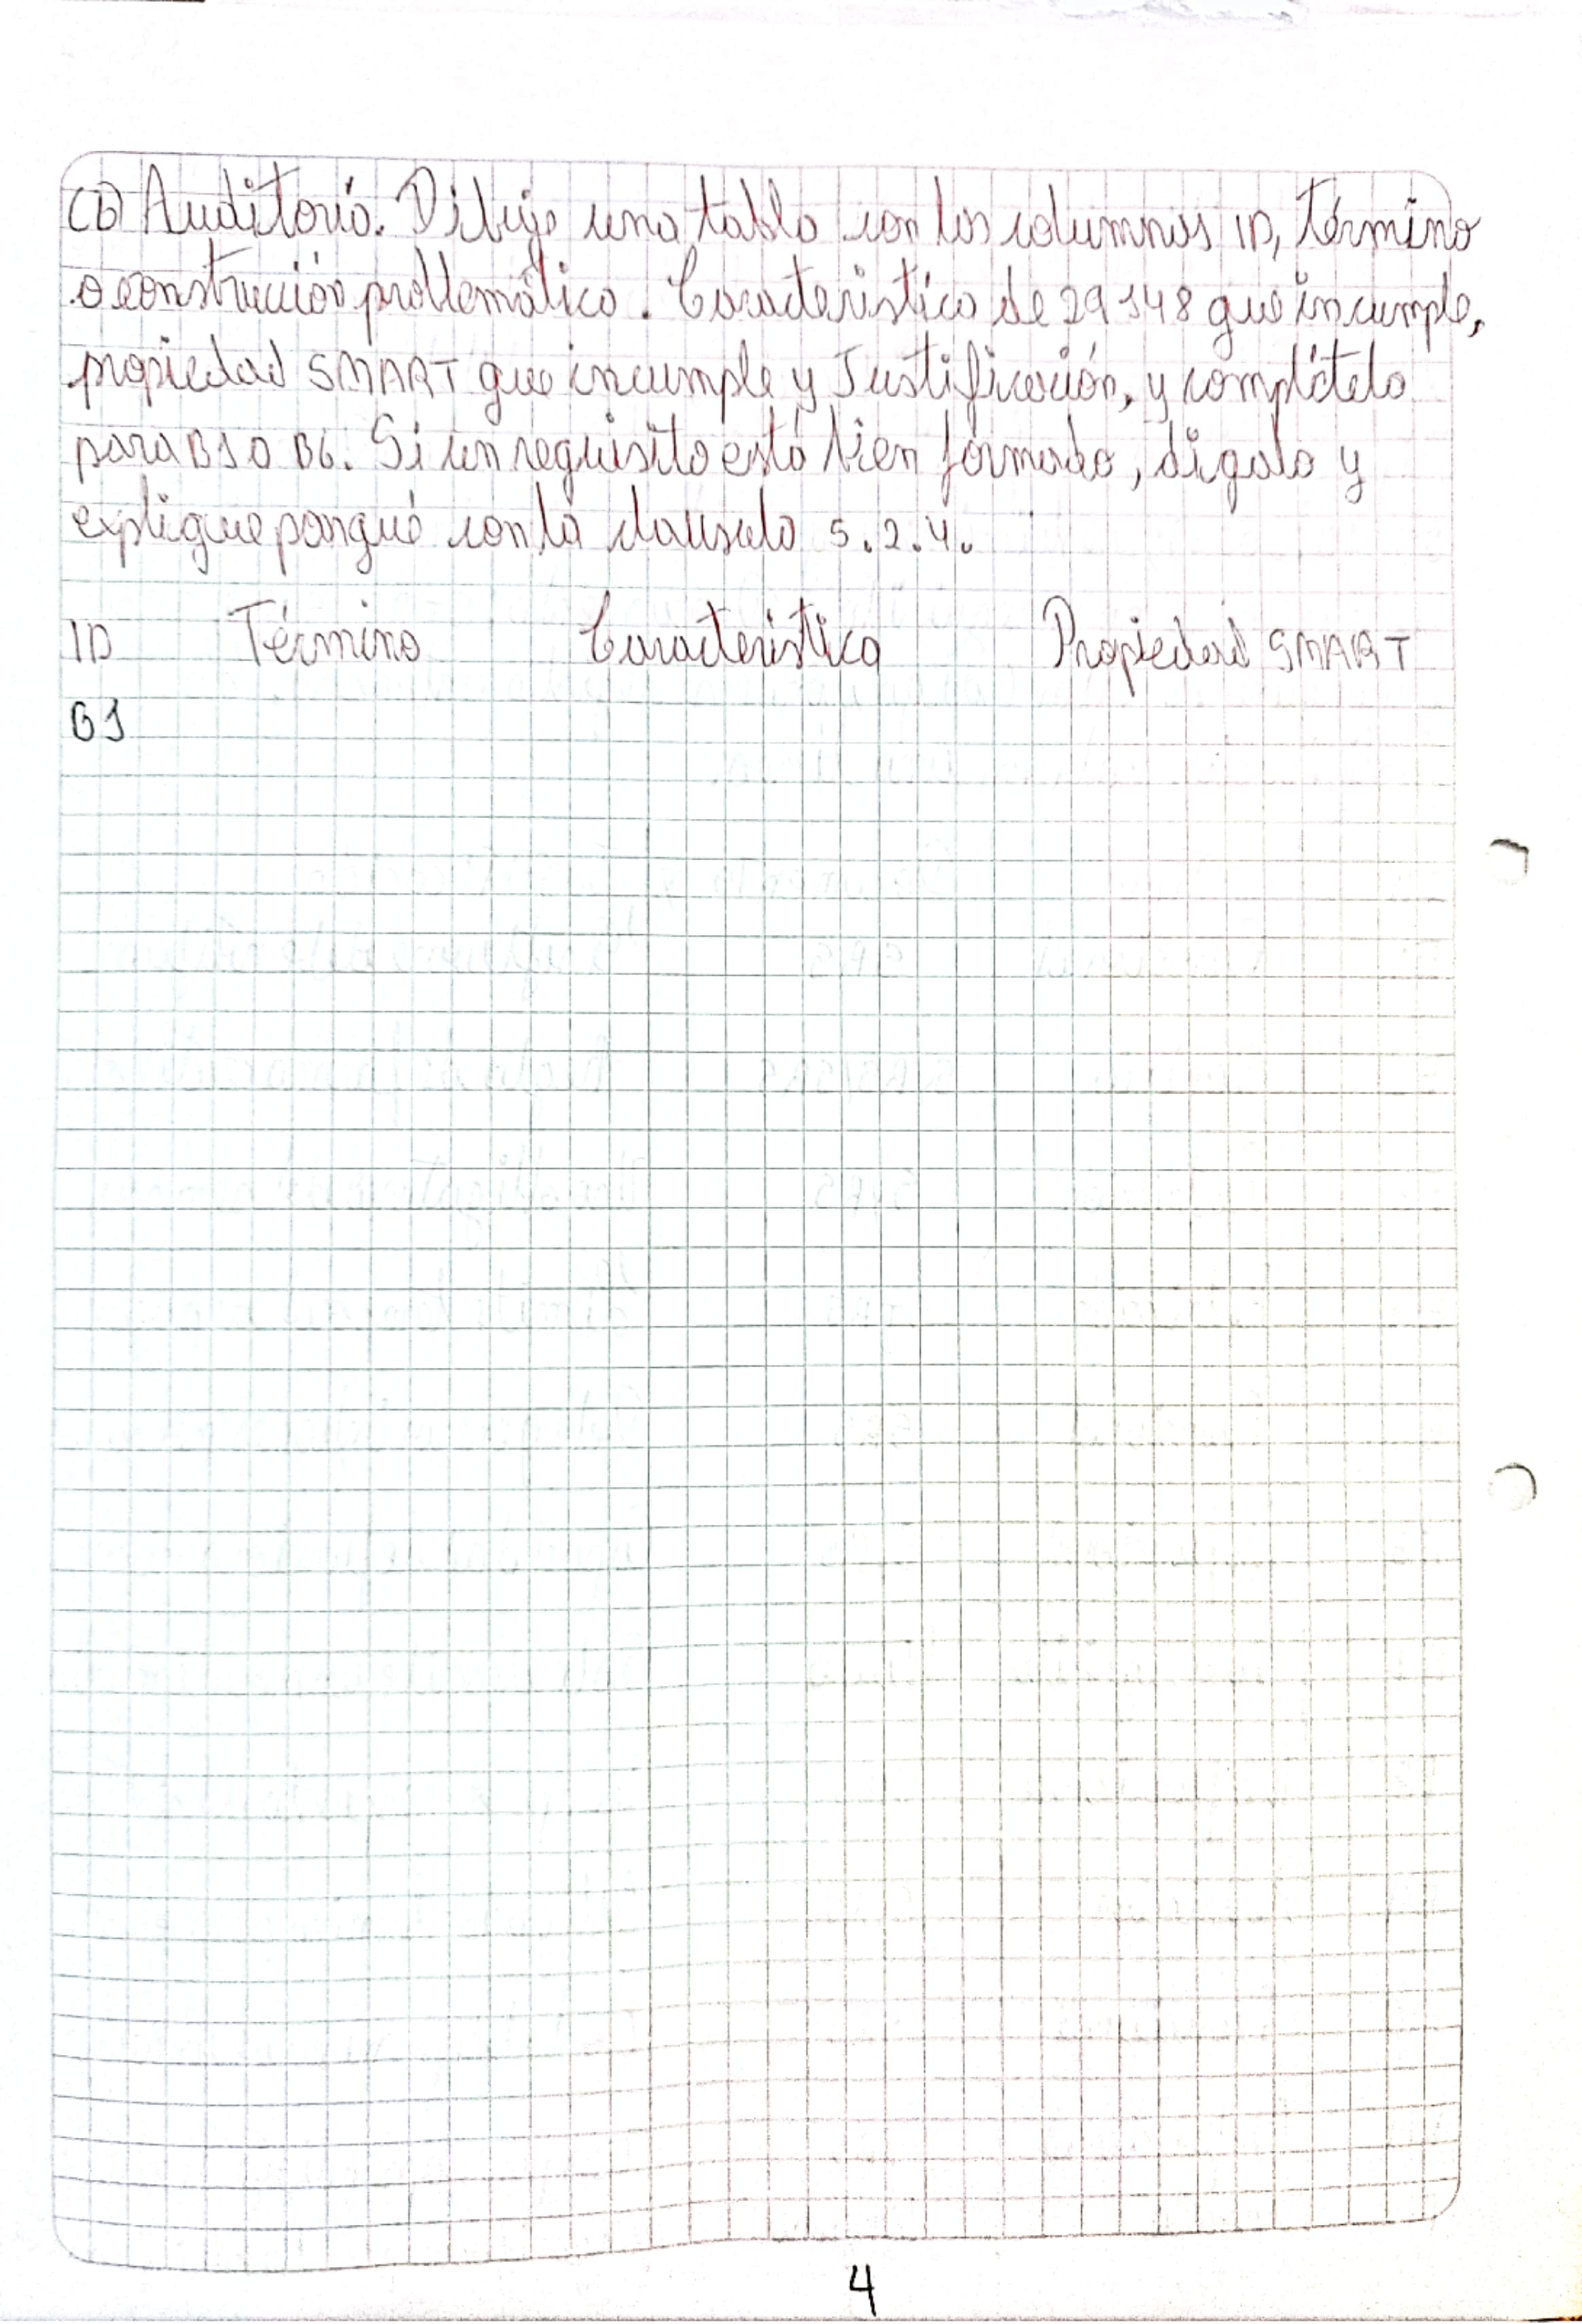
\includegraphics[width=0.85\textwidth,height=0.42\textheight,keepaspectratio]{evidencias/hoja-04.jpg}
\end{center}

\end{document}
